\begin{titre}[Les nombres]

\Titre{Intervalles de $\R$}{3}
\end{titre}


\begin{CpsCol}
\begin{description}
\item[$\square$] Représenter un intervalle de la droite numérique. 
\item[$\square$]  Déterminer si un nombre réel appartient à un intervalle donné.
\end{description}
\end{CpsCol}

\Rec{1}{FEA-11}


\begin{DefT}{Intervalle fermé}\index{Intervalle}
Un intervalle fermé de $\R$ est un sous-ensemble borné de $\R$, c'est à dire un ensemble de nombres compris entre deux valeurs réelles.
\end{DefT}

\begin{DefT}{Intervalle ouvert}\index{Intervalle}
Un intervalle ouvert de $\R$ est un sous-ensemble de $\R$ dont les bornes ne sont pas incluses dans l'ensemble, c'est à dire un ensemble de nombres compris entre deux valeurs réelles non comprises.
\end{DefT}

\begin{Ex}
\begin{enumerate}
\item On a représenté sur la droite des nombres réels tous les nombres réels $x$ tels que $-1 \leq x \leq 3$.

\begin{center}
\definecolor{ffxfqq}{rgb}{1.,0.4980392156862745,0.}
\begin{tikzpicture}[line cap=round,line join=round,>=triangle 45,x=1.0cm,y=1.0cm]
\draw[->,color=black] (-4.390839866186475,0.) -- (7.64974334956303,0.);
\foreach \x in {-4.,-3.,-2.,-1.,1.,2.,3.,4.,5.,6.,7.}
\draw[shift={(\x,0)},color=black] (0pt,2pt) -- (0pt,-2pt) node[below] {\footnotesize $\x$};
\draw[color=black] (0pt,-10pt) node[right] {\footnotesize $0$};
\clip(-4.390839866186475,-0.5880295569511441) rectangle (7.64974334956303,0.5863275715079787);
\draw [line width=2.4pt,color=ffxfqq] (-1.,0.)-- (3.,0.);
\draw [color=ffxfqq](-1.16,0.25) node[anchor=north west] {[};
\draw [color=ffxfqq](2.85,0.25) node[anchor=north west] {]};
\end{tikzpicture}
 \end{center} 
 
Cet intervalle est noté $[-1;3]$. Il est fermé.
 \item On a représenté sur la droite des nombres réels tous les nombres réels $x$ tels que $-1 < x < 3$.

\begin{center}
\definecolor{ffxfqq}{rgb}{1.,0.4980392156862745,0.}
\begin{tikzpicture}[line cap=round,line join=round,>=triangle 45,x=1.0cm,y=1.0cm]
\draw[->,color=black] (-4.390839866186475,0.) -- (7.64974334956303,0.);
\foreach \x in {-4.,-3.,-2.,-1.,1.,2.,3.,4.,5.,6.,7.}
\draw[shift={(\x,0)},color=black] (0pt,2pt) -- (0pt,-2pt) node[below] {\footnotesize $\x$};
\draw[color=black] (0pt,-10pt) node[right] {\footnotesize $0$};
\clip(-4.390839866186475,-0.5295569511441) rectangle (7.64974334956303,0.563275715079787);
\draw [line width=2.4pt,color=ffxfqq] (-1.,0.)-- (3.,0.);
\draw [color=ffxfqq](-1.16,0.25) node[anchor=north west] {]};
\draw [color=ffxfqq](2.85,0.25) node[anchor=north west] {[};
\end{tikzpicture}
 \end{center}
Cet intervalle ouvert est noté $]-1;3[$. Il est ouvert.

 \item On a représenté sur la droite des nombres réels tous les nombres réels $x$ tels que $x \geq -1$.


\begin{center}
\definecolor{ffxfqq}{rgb}{1.,0.4980392156862745,0.}
\begin{tikzpicture}[line cap=round,line join=round,>=triangle 45,x=1.0cm,y=1.0cm]
\draw[->,color=black] (-4.390839866186475,0.) -- (7.64974334956303,0.);
\foreach \x in {-4.,-3.,-2.,-1.,1.,2.,3.,4.,5.,6.,7.}
\draw[shift={(\x,0)},color=black] (0pt,2pt) -- (0pt,-2pt) node[below] {\footnotesize $\x$};
\draw[color=black] (0pt,-10pt) node[right] {\footnotesize $0$};
\clip(-4.390839866186475,-0.5880295569511441) rectangle (7.64974334956303,0.53275715079787);
\draw [line width=2.4pt,color=ffxfqq] (-1.,0.)-- (8.,0.);
\draw [color=ffxfqq](-1.16,0.25) node[anchor=north west] {[};
\end{tikzpicture}
 \end{center} 
Cet ensemble est noté $[-1 ; +\infty[$, cet intervalle est semi-ouvert.
\end{enumerate}
\end{Ex}

\begin{Rqs}
\begin{enumerate}
\item  $+ \infty$ se lit "plus l’infini". L'ensemble des nombres réels $\R$ est l’intervalle $]-\infty ; +\infty[ = \R$.
\item Un intervalle est une partie de $\R$ "sans trou", en "un seul morceau".
\item $+\infty$ et $-\infty$ ne sont pas des nombres. Ce ne sont que des notations (ce qui explique qu'ils soient toujours exclus).
\item Les intervalles correspondants aux quatre premières lignes du tableau sont dits bornés.
\item  Plus généralement, les différents types d'intervalles sont donnés dans le tableau ci-dessous (où $a$ et $b$ représentent deux réels, avec $a < b$).
\end{enumerate}
\end{Rqs}

\begin{center}
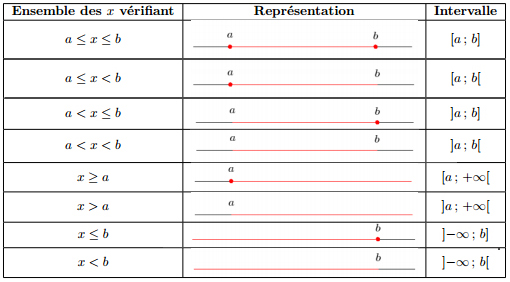
\includegraphics[scale=0.7]{cours4.jpg}
\end{center}


\EPC{1}{FEA-5}{Représenter}

\mini{
\EPC{1}{FEA-16}{Représenter}
}{
\EPC{0}{FEA-14}{Représenter}
}
\begin{DefT}{Intersection}\index{Ensemble!Intersection}
L'\textbf{intersection} de deux ensembles $A$ et $B$ est l'ensemble $A \cap B$ qui contient tous les éléments communs aux deux ensembles.
\end{DefT}

\begin{Rq}\index{Ensembles disjoints}
Deux ensembles sont disjoints lorsque $A \cap B = \oslash$. $\oslash$ est l'ensemble vide.\index{Ensemble!vide}
\end{Rq}


\begin{DefT}{Réunion}\index{Ensemble!Réunion}
La réunion de deux ensembles est l'ensemble $A \cup B$ qui contient tous les éléments des deux ensembles pris une seule fois.
\end{DefT}

\mini{
\EPC{1}{FEA-12}{Représenter}

}{
\EPC{0}{FEA-13}{Représenter}

}

\EPC{1}{FEA-93}{Représenter}

\EPC{0}{FEA-94}{Modéliser}

\EPCP{1}{FEA-92}{Représenter}

\EPC{1}{FEA-83}{Représenter. Chercher.}

\EPC{0}{FEA-83bis}{Représenter. Chercher.}

\paragraphe{Pour s'entrainer en autonomie}

\mini{

\EPC{0}{FEA-16B}{Représenter. Raisonner. Communiquer.}
}{

\EPC{0}{FEA-14B}{Représenter. Raisonner. Communiquer.}
 
}


\mini{

 
\EPC{0}{FEA-12B}{Représenter. Raisonner. Communiquer.}
 
}{

 
\EPC{0}{FEA-13B}{Représenter. Raisonner. Communiquer.}
 
}


\EPC{0}{FEA-108}{Représenter. Communiquer.}

 









